L'évolution d'un projet comme celui-ci peut prendre de nombreuses directions. Ajouter de nouvelles fonctionnalités, restructurer l'architecture pour améliorer l'efficacité, ou encore intégrer de nouvelles technologies pour résoudre les problèmes existants et explorer de nouvelles possibilités sont toutes des options viables. Voici quelques perspectives envisageables pour ce projet.

\section{Gestion des problèmes liés à WebRTC}

L'utilisation de WebRTC pour la communication en temps réel entre les utilisateurs est un élément clé de ce projet. Cependant, certains navigateurs ou réseaux peuvent bloquer cette technologie, rendant ainsi la fonctionnalité en temps réel non opérationnelle.

Une perspective pour résoudre ce problème pourrait être de proposer une alternative lorsque WebRTC n'est pas disponible. Par exemple, il pourrait être envisagé d'intégrer WebSocket ou d'autres technologies de serveur long-polling comme solution de secours. Cette amélioration nécessiterait une révision du réseau actuel et pourrait présenter des défis en termes de performances et de compatibilité, mais elle garantirait que les fonctionnalités en temps réel restent accessibles, même si WebRTC n'est pas une option.

\section{Stockage de données binaires}

Actuellement, le projet traite toutes les données à l'aide d'Automerge, qui utilise des CRDT pour gérer les conflits de manière décentralisée. Toutefois, il serait possible d'implémenter un système pour stocker des données binaires simples, comme des images ou des fichiers, qui n'ont pas besoin de la gestion de conflits offerte par les CRDT.

En ajoutant cette fonctionnalité, les utilisateurs pourraient partager et manipuler une plus grande variété de contenus. Cela nécessiterait toutefois une réflexion sur la manière de gérer ce nouveau type de données, notamment en termes de stockage, de partage et de synchronisation.

\section{Établissement d'un réseau maillé}

Une amélioration significative pourrait résider dans la mise en place d'un véritable réseau maillé, également appelé maillage en réseau. Dans un réseau maillé, chaque noeud est connecté à plusieurs autres, formant ainsi une structure décentralisée. Cette topologie de réseau est résiliente, car même si un noeud tombe en panne, les autres noeuds peuvent continuer à communiquer.

\begin{wrapfigure}{l}{0.30\textwidth}
    \centering
    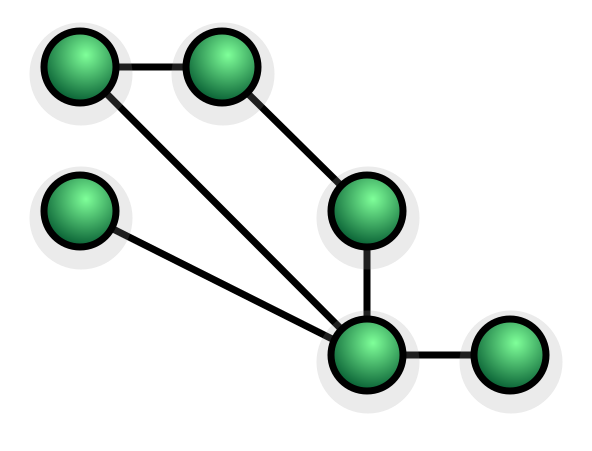
\includegraphics[width=0.30\textwidth]{\assetsdir/network-meshed.svg}
    \caption{Exemple de réseau maillé. (Source : Wikipedia\cite{TopologieMesh2023})}
    \label{fig:network-meshed}
\end{wrapfigure}

Cependant, un réseau maillé complet peut rapidement devenir complexe et difficile à gérer à mesure que le nombre de noeuds augmente. Par conséquent, une solution plus viable pourrait être d'organiser le réseau en clusters interconnectés, chaque cluster étant un petit réseau maillé en lui-même. Cela permettrait de conserver les avantages de la décentralisation et de la résilience offerts par un réseau maillé, tout en évitant la complexité qui pourrait survenir lors de l'ajout de nombreux noeuds.

Un tel réseau pourrait être construit en utilisant différentes technologies pour différents types de noeuds. Par exemple, WebRTC pourrait être utilisé pour les noeuds basés sur les navigateurs, WebSocket pour les noeuds serveurs, et TCP pour des connexions directes. Des ponts pourraient être utilisés pour connecter les différents types de noeuds, renforçant ainsi la robustesse du réseau.

Pour mettre en œuvre cette architecture réseau, le système actuel prévoit déjà le routage des données. Ainsi, il ne serait pas nécessaire de repenser entièrement l'architecture, mais plutôt de fusionner le client avec le serveur de signalisation, permettant à tous les clients d'agir également comme des routeurs.

\section{Amélioration du partage de contenu}

Actuellement, le partage d'accès aux contenus nécessite de connaître la clé publique des utilisateurs. Cela peut être déroutant, surtout pour les personnes qui ne sont pas familières avec ces concepts.

Une perspective d'amélioration pourrait être de simplifier ce processus de partage. Une solution pourrait être de mettre en place un système de "partage magique", où un lien unique serait généré pour chaque utilisateur. En cliquant sur ce lien, l'utilisateur serait automatiquement ajouté au système et aurait accès au contenu partagé. Cette amélioration rendrait le partage de contenu plus convivial et accessible à un public plus large.

Intégrer un tel système nécessiterait une refonte de l'interface utilisateur et du processus de partage des données, mais cela pourrait grandement améliorer l'expérience utilisateur en rendant le partage de contenu plus facile et intuitif.

\section{Audit de sécurité}

Étant donné l'utilisation extensive de la cryptographie dans ce projet, il est crucial d'assurer l'intégrité et la sécurité des données manipulées. Bien que l'application ait été conçue avec un souci de sécurité, il convient de souligner que le développement de ce projet n'a pas été effectué par un cryptographe professionnel.

Il serait donc vivement recommandé de faire auditer le code par un expert en sécurité informatique et en cryptographie. Cette étape permettrait de détecter d'éventuelles vulnérabilités et d'assurer la robustesse de l'application face à diverses attaques potentielles.

Une telle démarche d'audit ne vise pas seulement à identifier les faiblesses potentielles, mais aussi à valider les choix de conception en matière de sécurité. Elle offre également l'occasion d'obtenir des conseils d'experts sur les meilleures pratiques en matière de sécurité et de cryptographie.

En somme, un audit de sécurité serait une étape précieuse pour renforcer la confiance dans la sécurité de l'application et pour s'assurer qu'elle respecte les normes actuelles en matière de cryptographie et de protection des données.